\chapter{Measurement Data}
\label{app:measurement-tables}

This appendix gives the raw values behind the results of Chapter~\ref{chap:evaluation}. Each
measurement script writes a result file to \mbox{\texttt{docs/results/runs}}, and two scripts in
\mbox{\texttt{docs/diagrams/svg}} read those files: one builds the data of the charts and the other
the tables below, so a number in a chart and the same number here come from one record.
Table~\ref{tab:provenance} maps each table and figure of Chapter~\ref{chap:evaluation} to its result
file, its script and its table in this appendix.

\begin{table}[H]
\centering
\caption{Sources of the tables and figures of Chapter~\ref{chap:evaluation}}
\label{tab:provenance}
\footnotesize
\setlength{\tabcolsep}{4pt}
\begin{tabularx}{\textwidth}{>{\raggedright\arraybackslash}X >{\raggedright\arraybackslash}p{0.40\textwidth} >{\raggedright\arraybackslash}p{0.22\textwidth} >{\raggedright\arraybackslash}p{0.12\textwidth}}
\toprule
\textbf{IN CHAPTER 6} & \textbf{RESULT FILE} & \textbf{SCRIPT} & \textbf{RAW DATA} \\
\midrule
Figure~\ref{fig:ttff-steps} & \texttt{2026-11-04-v2-ttff.json} & \texttt{bench/ttff.mjs} & Table~\ref{tab:raw-ttff} \\
Table~\ref{tab:qoe-playback} & \texttt{2026-11-04-v2-qoe-unthrottled.json}, \texttt{2026-11-04-v2-qoe-fast3g.json}, \texttt{2026-11-04-v2-qoe-slow3g.json} & \texttt{qoe/collect.js} & Table~\ref{tab:raw-qoe} \\
Bandwidth drop, Section~\ref{sec:qoe-playback} & \texttt{2026-11-12-v2-qoe-drop.json} & \texttt{qoe/collect.js} & Table~\ref{tab:raw-qoe-drop} \\
Table~\ref{tab:bitrate-check} & \texttt{2026-11-04-v2-bitrate.json} & \texttt{bench/bitrate.mjs} & Table~\ref{tab:raw-bitrate} \\
Figure~\ref{fig:transcode-size}, Table~\ref{tab:transcode-results} & \texttt{2026-11-04-v2-s2b-resized.json} & \texttt{bench/transcode.mjs} & Table~\ref{tab:raw-transcode} \\
Real recording, Section~\ref{sec:size-evaluation} & \texttt{2026-11-03-v2-real-recording.json} & Execution history, read back & The file itself \\
Figure~\ref{fig:four-hour} & \texttt{2026-11-04-v2-s4-long.json}, \texttt{2026-11-24-v2-s4-long-rerun.json} & \texttt{bench/transcode.mjs} & Table~\ref{tab:raw-four-hour} \\
Damaged uploads, Section~\ref{sec:fault-evaluation} & \texttt{2026-11-11-v2-fault.json} & \texttt{bench/fault.mjs} & Table~\ref{tab:raw-fault} \\
Length limit, Section~\ref{sec:length-evaluation} & \texttt{2026-11-15-v2-length-limit.json} & Execution history, read back & The file itself \\
Figure~\ref{fig:burst} & \texttt{2026-11-04-v2-s3c-burst.json} & \texttt{bench/transcode.mjs} & Tables~\ref{tab:raw-burst} and~\ref{tab:raw-lambda} \\
Priority queues, Section~\ref{sec:priority-evaluation} & \texttt{2026-11-14-v2-priority.json} & Batch job history, read back & Table~\ref{tab:raw-priority} \\
Table~\ref{tab:api-load} & \texttt{2026-11-04-v2-api-final.json} & \texttt{bench/api-load.mjs} & Tables~\ref{tab:raw-api} and~\ref{tab:raw-lambda} \\
Table~\ref{tab:cost-comparison} & \texttt{2026-11-04-v2-prices.json}, \texttt{2026-11-05-v2-rekognition-price.json}, \texttt{2026-11-15-v2-transcribe-price.json} & \texttt{bench/cost.mjs}, AWS Price List Query API & Table~\ref{tab:raw-prices} \\
\bottomrule
\end{tabularx}
\end{table}

The scripts are under \mbox{\texttt{scripts}}. Every run was made on the production environment,
with the configuration of Chapter~\ref{chap:implementation}, except the run of the priority queues,
which was made on staging.

Percentiles use the nearest rank: the $p$-th percentile of $n$ sorted values is the value at position
$\lfloor p\,n \rfloor$, counted from zero and capped at the last one. With 20 values or fewer, the
95th percentile is therefore the largest value, which is why the columns 95TH PCT.\ and MAX agree in
Table~\ref{tab:raw-ttff} and in the bursts of 10 and 20 requests of Table~\ref{tab:raw-api}.

\section{Playback}

Table~\ref{tab:raw-ttff} breaks the requests of Figure~\ref{fig:ttff-steps} into their steps. The
first request found every cache cold; the other 19 followed it one after another.

% Generated by docs/diagrams/svg/build-v2-appendix-tables.mjs; do not edit by hand.
\begin{table}[H]
\centering
\caption{Requests before the first frame of the 720p rendition, in milliseconds; the first request and 19 that followed it}
\label{tab:raw-ttff}
\footnotesize
\begin{tabular}{l r r r r r r}
\toprule
\textbf{STEP} & \textbf{FIRST} & \textbf{MEAN} & \textbf{MEDIAN} & \textbf{95TH PCT.} & \textbf{MIN} & \textbf{MAX} \\
\midrule
Playback grant (API) & 479.4 & 122.3 & 121.6 & 137.5 & 108.2 & 137.5 \\
Master playlist (CDN) & 376.4 & 8.2 & 6.9 & 18.0 & 5.5 & 18.0 \\
Rendition playlist (CDN) & 128.3 & 10.8 & 8.1 & 56.9 & 5.7 & 56.9 \\
Key (API) & 175.4 & 150.0 & 144.2 & 216.6 & 125.2 & 216.6 \\
First segment (CDN) & 265.0 & 28.1 & 22.7 & 81.4 & 19.7 & 81.4 \\
\midrule
Total & 1424.9 & 319.5 & 307.5 & 435.2 & 288.4 & 435.2 \\
\bottomrule
\end{tabular}
\end{table}


Table~\ref{tab:raw-qoe} gives every playback run behind Table~\ref{tab:qoe-playback}. The rung is
read from the size of the video element's picture, so it is the rung on screen rather than the one
being downloaded; no run changed rung while it played. The bit rate is that of the rung on screen,
computed from the bytes of the segments of that rung which the run downloaded. Without throttling,
the player buffers the whole video, so the value equals the average of the rung over the whole
video (716~kbit/s at 480p, Table~\ref{tab:bitrate-check}). Under Fast~3G and Slow~3G it downloads
only the first one to two minutes, which are harder to compress than the rest, so the value lies
above that average: 809 against 716~kbit/s at 480p, and 258 against 249~kbit/s at 240p.

% Generated by docs/diagrams/svg/build-v2-appendix-tables.mjs; do not edit by hand.
\begin{table}[H]
\centering
\caption{Playback runs of 60 seconds under three network profiles}
\label{tab:raw-qoe}
\footnotesize
\begin{tabular}{l c r c r r l}
\toprule
\textbf{PROFILE} & \textbf{RUN} & \textbf{START-UP, S} & \textbf{STALLS} & \textbf{STALLED, S} & \textbf{KBIT/S} & \textbf{RUNG SHOWN} \\
\midrule
Unthrottled & 1 & 3.23 & 0 & 0.0 & 716 & 850$\times$480 \\
 & 2 & 3.10 & 0 & 0.0 & 716 & 850$\times$480 \\
 & 3 & 2.09 & 0 & 0.0 & 716 & 850$\times$480 \\
 & 4 & 1.98 & 0 & 0.0 & 716 & 850$\times$480 \\
 & 5 & 2.27 & 0 & 0.0 & 716 & 850$\times$480 \\
\midrule
Fast 3G & 1 & 6.07 & 0 & 0.0 & 809 & 850$\times$480 \\
 & 2 & 5.74 & 0 & 0.0 & 809 & 850$\times$480 \\
 & 3 & 5.70 & 0 & 0.0 & 809 & 850$\times$480 \\
 & 4 & 5.87 & 0 & 0.0 & 809 & 850$\times$480 \\
 & 5 & 8.89 & 0 & 0.0 & 795 & 850$\times$480 \\
\midrule
Slow 3G & 1 & 9.13 & 0 & 0.0 & 258 & 426$\times$240 \\
 & 2 & 9.01 & 0 & 0.0 & 258 & 426$\times$240 \\
 & 3 & 9.29 & 0 & 0.0 & 258 & 426$\times$240 \\
 & 4 & 8.88 & 0 & 0.0 & 258 & 426$\times$240 \\
 & 5 & 8.90 & 0 & 0.0 & 258 & 426$\times$240 \\
\bottomrule
\end{tabular}
\end{table}


Table~\ref{tab:raw-qoe-drop} gives the runs with a bandwidth drop. The drop is applied twenty seconds
after playback is requested. A lower rung counts as requested at the first segment request below the
highest rung requested so far, and as on screen at the first change of the picture to a rung below
the highest shown so far.

% Generated by docs/diagrams/svg/build-v2-appendix-tables.mjs; do not edit by hand.
\begin{table}[H]
\centering
\caption{Playback runs of 90 seconds that start on Fast 3G and drop to Slow 3G after 20 seconds: the rung shown before the drop, and the seconds from the drop until a lower rung was asked for and shown}
\label{tab:raw-qoe-drop}
\footnotesize
\begin{tabular}{c r c r c r c r}
\toprule
\textbf{RUN} & \textbf{START-UP} & \textbf{BEFORE} & \textbf{ASKED} & \textbf{RUNG} & \textbf{SHOWN} & \textbf{RUNG} & \textbf{STALLS} \\
\midrule
1 & 5.94 & 480p & 8.6 & 240p & 20.2 & 240p & 0 \\
2 & 5.83 & 480p & 8.5 & 240p & 20.2 & 240p & 0 \\
3 & 6.22 & 480p & 8.9 & 240p & 20.4 & 240p & 0 \\
4 & 5.94 & 480p & 8.5 & 360p & 20.6 & 360p & 0 \\
5 & 6.05 & 480p & 8.7 & 240p & 20.3 & 240p & 0 \\
\bottomrule
\end{tabular}
\end{table}


Table~\ref{tab:raw-bitrate} compares the playlists of the three measured videos with their segments.
The first video is the recording of Table~\ref{tab:bitrate-check}; the other two are synthetic test
patterns.

% Generated by docs/diagrams/svg/build-v2-appendix-tables.mjs; do not edit by hand.
\begin{table}[H]
\centering
\caption{Declared (decl.) and delivered (deliv.) bit rate of three videos, in kbit/s; count of segments, and length of a segment without the last one}
\label{tab:raw-bitrate}
\footnotesize
\setlength{\tabcolsep}{4pt}
\begin{tabular}{l l r r r r r r}
\toprule
 & & & \multicolumn{2}{c}{\textbf{PEAK}} & \multicolumn{2}{c}{\textbf{AVERAGE}} & \\
\cmidrule(lr){4-5} \cmidrule(lr){6-7}
\textbf{VIDEO} & \textbf{RUNG} & \textbf{COUNT} & \textbf{DECL.} & \textbf{DELIV.} & \textbf{DECL.} & \textbf{DELIV.} & \textbf{LENGTH, S} \\
\midrule
Recording & 144p & 47 & 201 & 201 & 154 & 154 & 5.97--6.01 \\
 & 240p & 47 & 408 & 408 & 249 & 249 & 5.97--6.01 \\
 & 360p & 47 & 688 & 688 & 420 & 420 & 5.97--6.01 \\
 & 480p & 47 & 1178 & 1178 & 716 & 716 & 5.97--6.01 \\
 & 720p & 47 & 2443 & 2443 & 1578 & 1578 & 5.97--6.01 \\
 & 1080p & 47 & 4933 & 4933 & 3562 & 3562 & 5.97--6.01 \\
\midrule
Test pattern A & 144p & 31 & 181 & 181 & 59 & 59 & 6.00--6.00 \\
 & 240p & 31 & 253 & 253 & 74 & 74 & 6.00--6.00 \\
 & 360p & 31 & 334 & 334 & 89 & 89 & 6.00--6.00 \\
 & 480p & 31 & 406 & 406 & 122 & 122 & 6.00--6.00 \\
 & 720p & 31 & 569 & 569 & 189 & 189 & 6.00--6.00 \\
 & 1080p & 31 & 750 & 750 & 274 & 274 & 6.00--6.00 \\
\midrule
Test pattern B & 144p & 20 & 61 & 61 & 59 & 59 & 6.00--6.00 \\
 & 240p & 20 & 74 & 74 & 73 & 73 & 6.00--6.00 \\
 & 360p & 20 & 91 & 91 & 88 & 88 & 6.00--6.00 \\
 & 480p & 20 & 122 & 122 & 122 & 122 & 6.00--6.00 \\
 & 720p & 20 & 190 & 190 & 188 & 188 & 6.00--6.00 \\
 & 1080p & 20 & 278 & 278 & 274 & 274 & 6.00--6.00 \\
\bottomrule
\end{tabular}
\end{table}


\begin{table}[H]
\centering
\caption{Declared and delivered bit rate of a production recording, in kbit/s (47 segments per rung)}
\label{tab:bitrate-check}
\small
\begin{tabular}{l l r r r r}
\toprule
 & & \multicolumn{2}{c}{\textbf{PEAK}} & \multicolumn{2}{c}{\textbf{AVERAGE}} \\
\cmidrule(lr){3-4} \cmidrule(lr){5-6}
\textbf{RUNG} & \textbf{SIZE} & \textbf{DECLARED} & \textbf{DELIVERED} & \textbf{DECLARED} & \textbf{DELIVERED} \\
\midrule
144p  & 256$\times$144   & 201  & 201  & 154  & 154 \\
240p  & 426$\times$240   & 408  & 408  & 249  & 249 \\
360p  & 638$\times$360   & 688  & 688  & 420  & 420 \\
480p  & 850$\times$480   & 1178 & 1178 & 716  & 716 \\
720p  & 1276$\times$720  & 2443 & 2443 & 1578 & 1578 \\
1080p & 1912$\times$1080 & 4933 & 4933 & 3562 & 3562 \\
\bottomrule
\end{tabular}
\end{table}

\section{Transcoding}

Table~\ref{tab:raw-transcode} lists the twelve runs behind Figure~\ref{fig:transcode-size}. Intake is
the time from the end of the upload to the end of the probe, and the start column is the time
from the end of the upload until the first Fargate task starts, so it includes the intake. Analysis
runs in parallel with encoding, so the columns do not add up to the total.

% Generated by docs/diagrams/svg/build-v2-appendix-tables.mjs; do not edit by hand.
\begin{table}[H]
\centering
\caption{Transcoding runs by file size, in seconds from the end of the upload; intake ends with the probe, and start is when the first task starts; encoding is the single job or the chunk array}
\label{tab:raw-transcode}
\footnotesize
\setlength{\tabcolsep}{2.5pt}
\begin{tabular}{l c c r r r r r r r}
\toprule
\textbf{SOURCE} & \textbf{RUN} & \textbf{CHUNKS} & \textbf{INTAKE} & \textbf{START} & \textbf{ANALYSE} & \textbf{ENCODE} & \textbf{STITCH} & \textbf{READY} & \textbf{vCPU-S} \\
\midrule
36 s clip & 1 & -- & 24.9 & 55.2 & 24.9 & 30.4 & -- & 112.1 & 171 \\
 & 2 & -- & 22.2 & 55.6 & 24.1 & 30.0 & -- & 94.1 & 168 \\
 & 3 & -- & 22.2 & 45.3 & 24.4 & 28.0 & -- & 110.6 & 161 \\
\midrule
100 MB & 1 & -- & 22.4 & 42.8 & 32.9 & 68.1 & -- & 122.2 & 611 \\
 & 2 & -- & 21.7 & 57.0 & 35.1 & 89.8 & -- & 148.4 & 789 \\
 & 3 & -- & 22.1 & 48.4 & 39.5 & 62.8 & -- & 119.6 & 581 \\
\midrule
500 MB & 1 & 10 & 11.2 & 33.8 & 76.3 & 111.2 & 1.5 & 148.7 & 3757 \\
 & 2 & 10 & 23.2 & 41.8 & 76.5 & 101.8 & 0.9 & 146.9 & 3120 \\
 & 3 & 10 & 22.2 & 41.1 & 92.2 & 102.4 & 0.7 & 146.9 & 3477 \\
\midrule
1 GB & 1 & 18 & 22.8 & 45.7 & 90.8 & 241.1 & 1.7 & 291.0 & 7853 \\
 & 2 & 18 & 13.5 & 35.2 & 66.3 & 245.1 & 1.5 & 286.6 & 7328 \\
 & 3 & 18 & 6.6 & 29.2 & 74.7 & 251.6 & 0.9 & 284.0 & 7226 \\
\bottomrule
\end{tabular}
\end{table}


% Generated by docs/diagrams/svg/build-v2-appendix-tables.mjs; do not edit by hand.
\begin{table}[H]
\centering
\caption{Steps of the four-hour video in three runs, 5.259 GiB, 48 chunks of 4 vCPUs, times in seconds}
\label{tab:raw-four-hour}
\small
\begin{tabular}{l r r r}
\toprule
\textbf{STEP OR QUANTITY} & \textbf{4 NOV} & \textbf{24 NOV, 1} & \textbf{24 NOV, 2} \\
\midrule
Upload of the source & 132.6 & 96.6 & 100.2 \\
Intake: workflow start and probe & 12.8 & 9.5 & 26.4 \\
End of upload to the first task & 33.9 & 40.3 & 48.0 \\
Analyse, in parallel with the audio & 107.3 & 98.9 & 105.0 \\
Audio of the whole video & 649.2 & 470.7 & 557.0 \\
Chunk array, 48 chunks & 1591.6 & 1681.8 & 1697.4 \\
Stitch & 2.3 & 2.1 & 2.1 \\
Publish & 0.3 & 0.3 & 0.2 \\
\midrule
End of upload to ready & 2298.9 & 2222.1 & 2331.2 \\
Work of all tasks, vCPU-s & 67285 & 65631 & 65309 \\
Tasks on Spot and On-Demand & 27 and 23 & 29 and 21 & 28 and 22 \\
\bottomrule
\end{tabular}
\end{table}


Table~\ref{tab:raw-fault} lists the uploads of damaged files of Section~\ref{sec:fault-evaluation}.
The image is the transcoder release that ran; attempts are those of the failed step, and for a Batch
step the exit codes of its attempts. The first run of the truncated file failed on an error of the
Batch API, not of the file, and the second shows the defect that the release 9f43f64 fixed.

% Generated by docs/diagrams/svg/build-v2-appendix-tables.mjs; do not edit by hand.
\begin{table}[H]
\centering
\caption{Uploads of damaged files on production; time in seconds from the end of the upload to the end of the workflow}
\label{tab:raw-fault}
\footnotesize
\begin{tabular}{l l l l l r}
\toprule
\textbf{FILE} & \textbf{IMAGE} & \textbf{FAILED STEP} & \textbf{ATTEMPTS} & \textbf{RESULT} & \textbf{TIME} \\
\midrule
Random bytes & 54da21d & Probe & 1 & \status{error} & 34.9 \\
Truncated, run 1 & 54da21d & Encode & 1 & \status{error} & 26.2 \\
Truncated, run 2 & 54da21d & -- & -- & \status{ready} & 141.1 \\
Truncated, after the fix & 9f43f64 & Encode & 1 (exit 3) & \status{error} & 154.2 \\
\bottomrule
\end{tabular}
\end{table}


\begin{figure}[htbp]
\centering
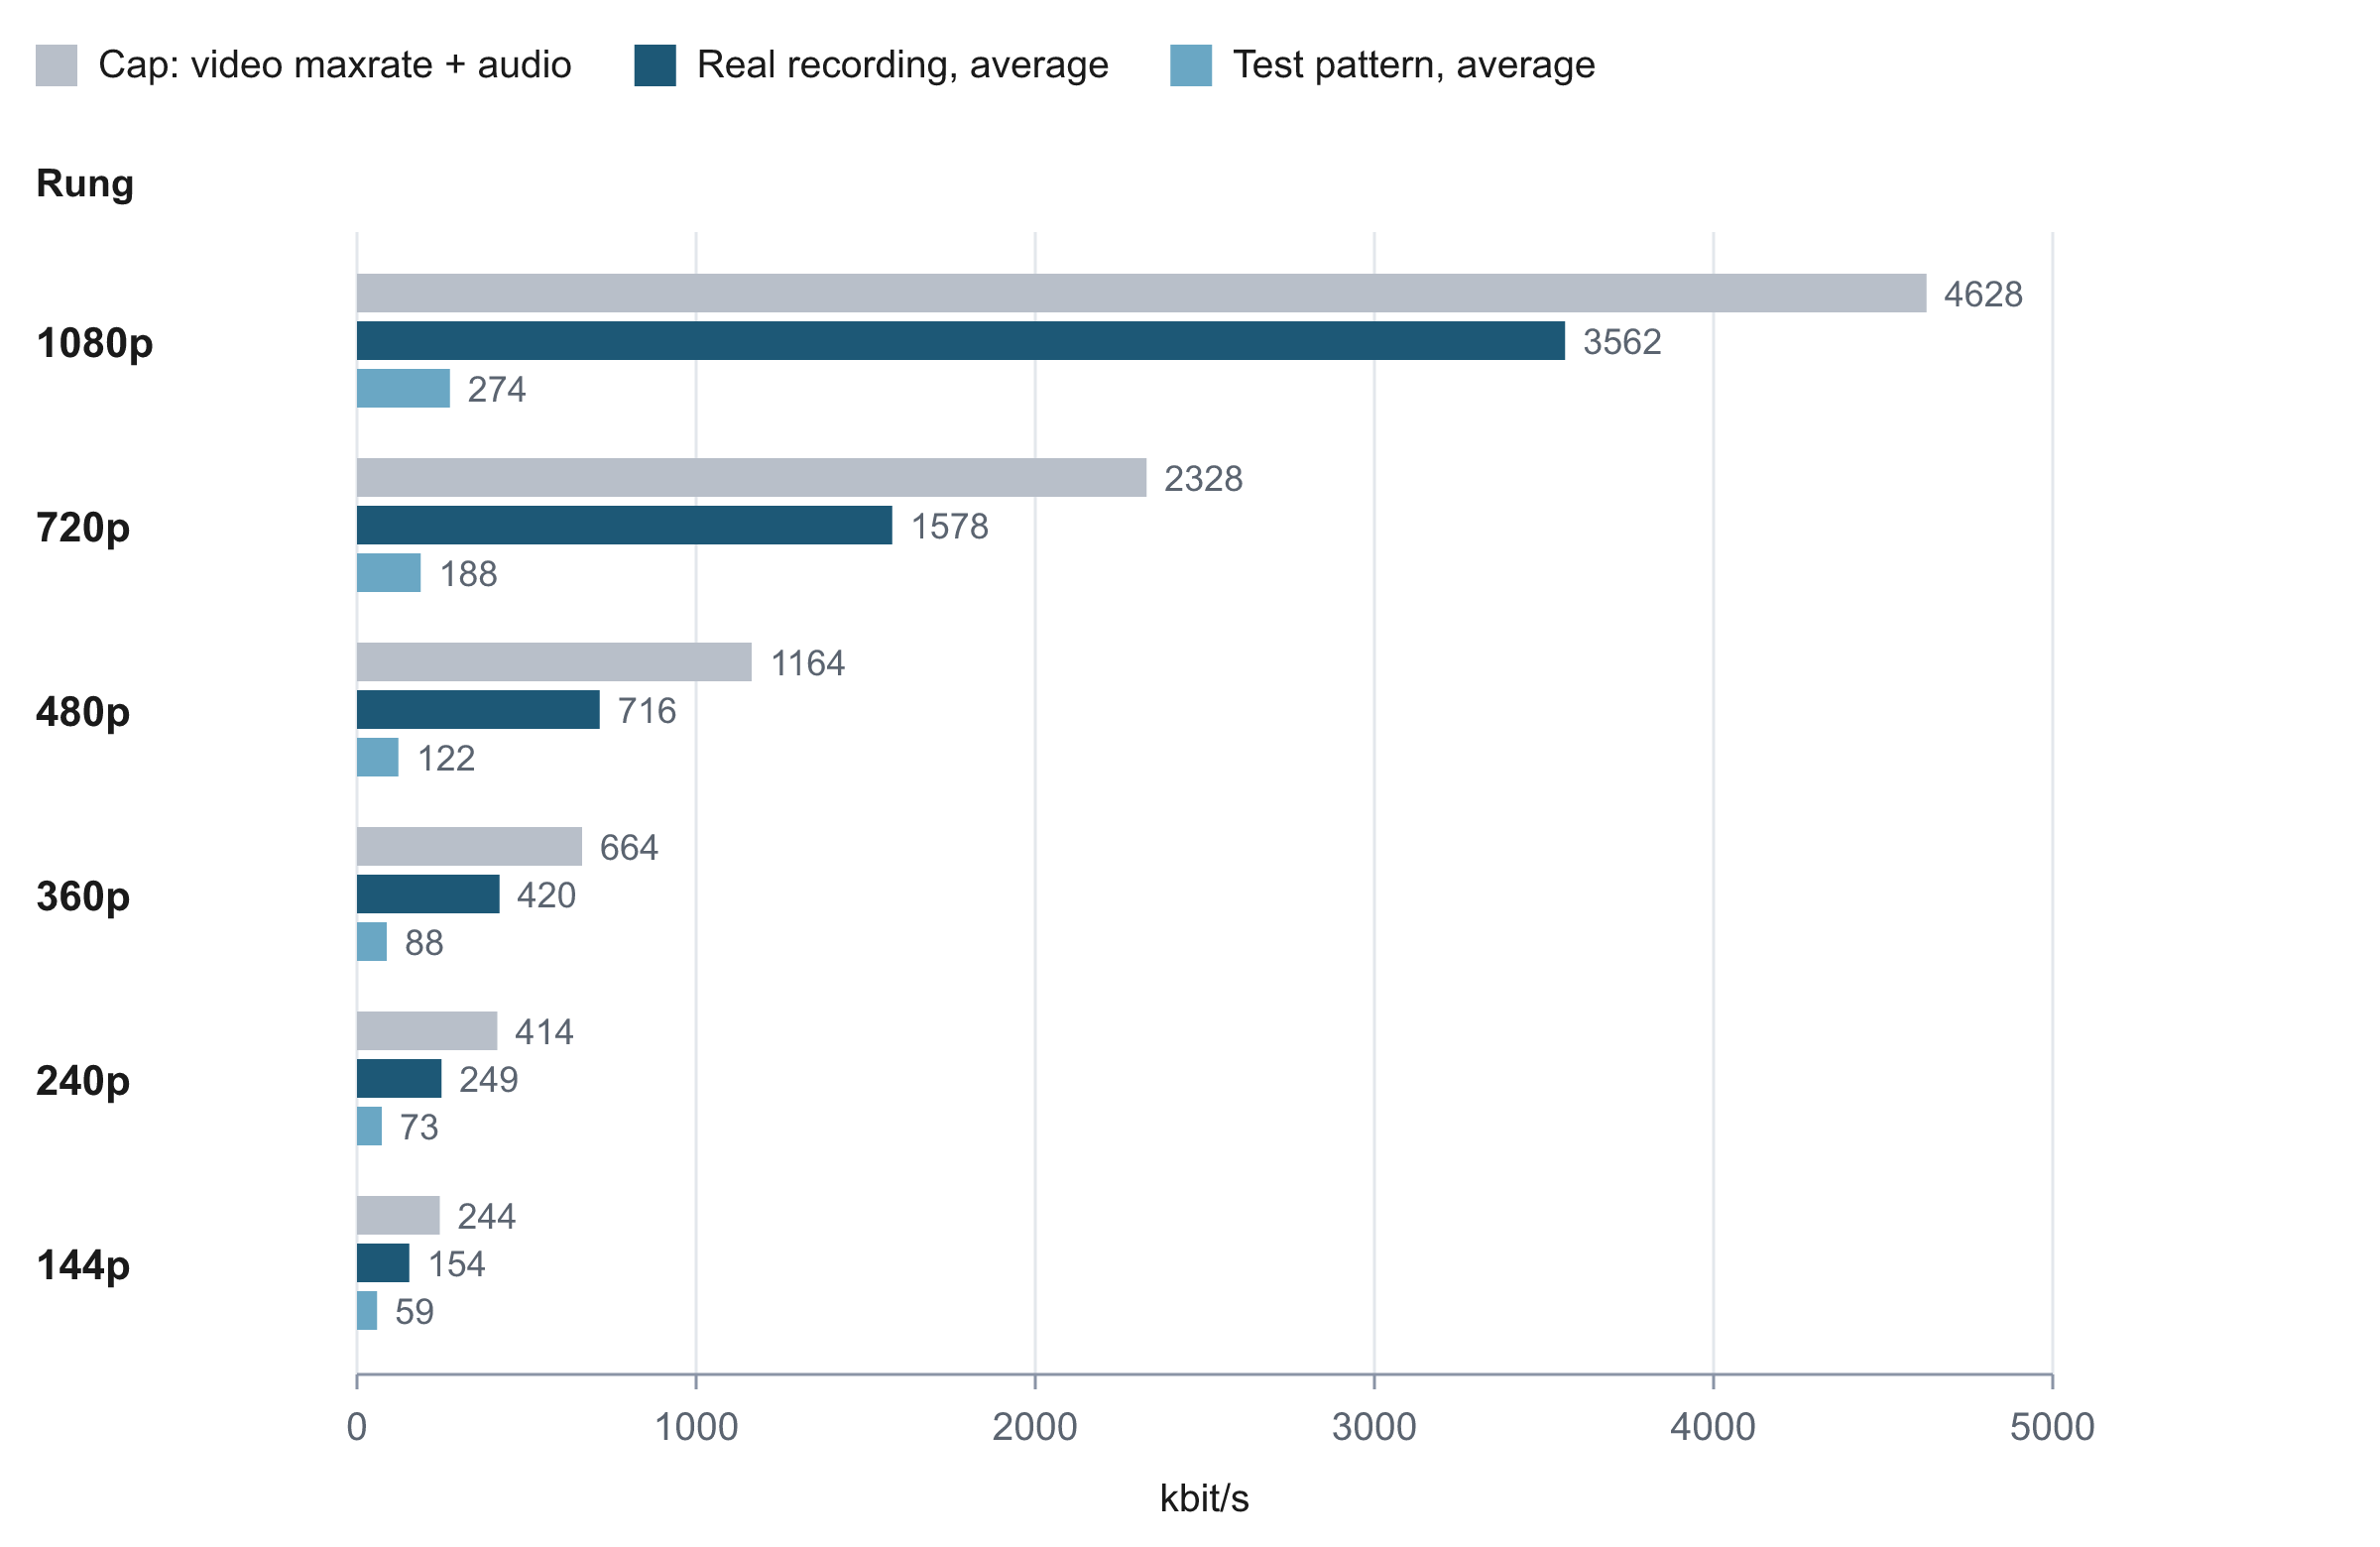
\includegraphics[width=\textwidth]{images/24-chart-ladder.png}
\caption{\textit{Cap of each rung against the measured average bit rate of two production videos}}
\label{fig:ladder}
\end{figure}

\begin{table}[H]
\centering
\caption{Transcoding time by file size, three runs each}
\label{tab:transcode-results}
\small
\begin{tabularx}{\textwidth}{>{\raggedright\arraybackslash}X >{\raggedright\arraybackslash}p{0.12\textwidth} >{\raggedleft\arraybackslash}p{0.13\textwidth} >{\raggedleft\arraybackslash}p{0.13\textwidth} >{\raggedleft\arraybackslash}p{0.16\textwidth}}
\toprule
\textbf{SOURCE} & \textbf{PATH} & \textbf{TO READY, MEDIAN} & \textbf{RANGE} & \textbf{vCPU-s PER SECOND OF SOURCE} \\
\midrule
36 s clip, 640$\times$360 & Single & 111 s & 94--112 s & 4.67 \\
100 MB, 2 min, 1080p & Single & 122 s & 120--148 s & 5.09 \\
500 MB, 10 min, 1080p & 10 chunks & 147 s & 147--149 s & 5.80 \\
1 GB, 26.7 min, 1080p & 18 chunks & 287 s & 284--291 s & 4.58 \\
\bottomrule
\end{tabularx}
\end{table}

\section{Load}

Table~\ref{tab:raw-burst} summarises the 89 videos of Figure~\ref{fig:burst} that reached
\status{ready} with a timing record; the three that became ready after a refused completion call
have none, because the measurement tool stopped following them, and the \texttt{follow\_up} field
of the result file records their executions. Table~\ref{tab:raw-lambda} gives the log of the API function during that run and
during the API run of Table~\ref{tab:raw-api}.

% Generated by docs/diagrams/svg/build-v2-appendix-tables.mjs; do not edit by hand.
\begin{table}[H]
\centering
\caption{One hundred simultaneous uploads: 92 ready (89 timed, 3 of the 3 with a refused completion call) and 8 refused at creation; times of the timed videos in seconds}
\label{tab:raw-burst}
\small
\begin{tabular}{l r r r r}
\toprule
\textbf{TIME PER VIDEO} & \textbf{MIN} & \textbf{MEDIAN} & \textbf{95TH PCT.} & \textbf{MAX} \\
\midrule
End of upload to the first task & 24.9 & 292.3 & 583.5 & 606.6 \\
First task to ready & 28.4 & 41.0 & 79.8 & 153.9 \\
End of upload to ready & 57.0 & 331.2 & 615.1 & 638.4 \\
\midrule
\multicolumn{5}{l}{Tasks run on Spot and On-Demand: 96 and 82} \\
\bottomrule
\end{tabular}
\end{table}


% Generated by docs/diagrams/svg/build-v2-appendix-tables.mjs; do not edit by hand.
\begin{table}[H]
\centering
\caption{Latency of read requests through the Worker by phase, in milliseconds}
\label{tab:raw-api}
\footnotesize
\begin{tabular}{l r r r r r r r}
\toprule
\textbf{PHASE} & \textbf{SENT} & \textbf{200} & \textbf{MEAN} & \textbf{MEDIAN} & \textbf{95TH PCT.} & \textbf{MAX} & \textbf{WALL} \\
\midrule
Sequential, warm & 40 & 40 & 166 & 156 & 263 & 279 & -- \\
Burst of 10 & 10 & 10 & 2347 & 2730 & 2916 & 2916 & 2922 \\
Burst of 20 & 20 & 20 & 1540 & 1336 & 2682 & 2682 & 2686 \\
Burst of 40 & 40 & 40 & 2217 & 2547 & 3382 & 3390 & 3396 \\
Burst of 80 & 80 & 80 & 4280 & 4395 & 5663 & 5682 & 5708 \\
\bottomrule
\end{tabular}
\end{table}


% Generated by docs/diagrams/svg/build-v2-appendix-tables.mjs; do not edit by hand.
\begin{table}[H]
\centering
\caption{Log of the API function during the API run and the burst of uploads; times in milliseconds}
\label{tab:raw-lambda}
\small
\begin{tabular}{l r r}
\toprule
\textbf{QUANTITY} & \textbf{API RUN} & \textbf{BURST OF UPLOADS} \\
\midrule
Invocations & 193 & -- \\
Most instances at once & -- & 80 \\
New instances & 79 & 80 \\
Start-up of an instance, mean & 1101 & 1106 \\
Start-up of an instance, max & 1248 & 1210 \\
Handler, median & 1394 & 512 \\
Handler, 95th percentile & 3938 & 7803 \\
Handler, max & 4077 & 8846 \\
Throttled invocations & -- & 56 \\
Failed invocations & -- & 0 \\
\bottomrule
\end{tabular}
\end{table}


Table~\ref{tab:raw-priority} lists the fourteen videos of Section~\ref{sec:priority-evaluation} in the
order their first job started. Upload is the order in which the videos were uploaded; queued is when
the first job of the video entered its queue, started when the first of its two jobs started, and
done when the last one ended, all in seconds from the first job of the run.

% Generated by docs/diagrams/svg/build-v2-appendix-tables.mjs; do not edit by hand.
\begin{table}[H]
\centering
\caption{Fourteen videos of 60 seconds on staging (8 + 8 vCPUs), in the order their first job started; seconds from the first job of the run}
\label{tab:raw-priority}
\footnotesize
\begin{tabular}{c c l l r r r r}
\toprule
\textbf{START} & \textbf{UPLOAD} & \textbf{ACCOUNT} & \textbf{QUEUE} & \textbf{QUEUED} & \textbf{STARTED} & \textbf{WAIT} & \textbf{DONE} \\
\midrule
1 & 1 & Free, first batch & main & 0.0 & 23.2 & 23.2 & 67.2 \\
2 & 2 & Free, first batch & main & 9.0 & 30.5 & 21.4 & 59.5 \\
3 & 7 & Free, first batch & main & 9.7 & 33.7 & 24.0 & 91.2 \\
4 & 6 & Free, first batch & main & 10.1 & 79.0 & 68.9 & 126.9 \\
5 & 9 & Plus & priority & 40.0 & 85.4 & 45.4 & 124.0 \\
6 & 12 & Plus & priority & 41.8 & 99.6 & 57.7 & 171.5 \\
7 & 3 & Free, first batch & main & 11.2 & 134.1 & 123.0 & 181.5 \\
8 & 4 & Free, first batch & main & 11.5 & 140.2 & 128.7 & 226.7 \\
9 & 10 & Plus & priority & 44.5 & 144.5 & 100.0 & 223.7 \\
10 & 13 & Plus & priority & 59.3 & 184.2 & 124.8 & 274.1 \\
11 & 5 & Free, first batch & main & 11.6 & 194.4 & 182.8 & 230.1 \\
12 & 8 & Free, first batch & main & 12.0 & 224.4 & 212.5 & 277.8 \\
13 & 14 & Free, second batch & main & 60.2 & 246.8 & 186.6 & 289.8 \\
14 & 11 & Free, second batch & main & 44.9 & 289.6 & 244.7 & 347.5 \\
\bottomrule
\end{tabular}
\end{table}


\begin{table}[H]
\centering
\caption{Latency of read requests through the Worker, in milliseconds}
\label{tab:api-load}
\small
\begin{tabular}{l r r r r}
\toprule
\textbf{PHASE} & \textbf{REQUESTS} & \textbf{ANSWERED 200} & \textbf{MEDIAN} & \textbf{95TH PERCENTILE} \\
\midrule
Sequential, warm & 40 & 40 & 156  & 263  \\
Burst of 10      & 10 & 10 & 2730 & 2916 \\
Burst of 20      & 20 & 20 & 1336 & 2682 \\
Burst of 40      & 40 & 40 & 2547 & 3382 \\
Burst of 80      & 80 & 80 & 4395 & 5663 \\
\bottomrule
\end{tabular}
\end{table}

\section{Prices}

Table~\ref{tab:raw-prices} gives the list prices read for the cost comparison of
Table~\ref{tab:cost-comparison} and for the automatic captions.

% Generated by docs/diagrams/svg/build-v2-appendix-tables.mjs; do not edit by hand.
\begin{table}[H]
\centering
\caption{List prices in Singapore, in USD}
\label{tab:raw-prices}
\small
\begin{tabular}{l r l}
\toprule
\textbf{ITEM} & \textbf{PRICE} & \textbf{UNIT} \\
\midrule
Fargate, vCPU & 0.05056 & per vCPU-hour \\
Fargate, memory & 0.00553 & per GB-hour \\
EC2 t3.medium, 2 vCPUs, 4 GiB & 0.0528 & per hour \\
EC2 t3.xlarge, 4 vCPUs, 16 GiB & 0.2112 & per hour \\
EC2 c6i.xlarge, 4 vCPUs, 8 GiB & 0.196 & per hour \\
EC2 c6i.2xlarge, 8 vCPUs, 16 GiB & 0.392 & per hour \\
Lambda, requests & 0.20 & per million requests \\
Lambda, compute & 0.0000166667 & per GB-second \\
S3 Standard & 0.024 & per GB-month \\
Rekognition, moderation & 0.0013 & per image \\
Transcribe, batch & 0.006 & per minute of audio, billed per second \\
\bottomrule
\end{tabular}
\end{table}

